\documentclass[conference]{IEEEtran}
\IEEEoverridecommandlockouts
% The preceding line is only needed to identify funding in the first footnote. If that is unneeded, please comment it out.
%Template version as of 6/27/2024

\usepackage{cite}
\usepackage{amsmath,amssymb,amsfonts}
\usepackage{algorithmic}
\usepackage{graphicx}
\usepackage{textcomp}
\usepackage{xcolor}
\def\BibTeX{{\rm B\kern-.05em{\sc i\kern-.025em b}\kern-.08em
    T\kern-.1667em\lower.7ex\hbox{E}\kern-.125emX}}
\begin{document}

\title{ATLAS: Adaptive Tool Learning with Agent Synthesis through Memory-Augmented Multi-Component LLMs}

\author{\IEEEauthorblockN{Yousha Saibi}
\IEEEauthorblockA{\textit{Department of Computer Science} \\
\textit{FAST NUCES}}
\and
\IEEEauthorblockN{Abdullah}
\IEEEauthorblockA{\textit{Department of Computer Science} \\
\textit{FAST NUCES}}
}

\maketitle

\begin{abstract}
Large Language Models (LLMs) have demonstrated remarkable capabilities in tool use and complex reasoning tasks, yet deploying large-scale models remains computationally expensive and inaccessible to many practitioners. Recent advances in modular architectures have shown that decomposing tool-use tasks into specialized components using smaller LLMs can achieve competitive performance. However, existing multi-component approaches suffer from lack of inter-component memory sharing, leading to context loss, redundant reasoning, and failure to learn from past interactions. In this paper, we propose ATLAS (Adaptive Tool Learning with Agent Synthesis), a memory-augmented multi-component framework that enhances small-LLM tool learning through episodic memory and adaptive routing. We demonstrate two instantiations: rules-based complexity routing and LLM-based planning with Llama 3.1 (8B). On ToolBench (500 cases), ATLAS achieves 97.4\% tool match with memory-augmented retrieval; on API-Bank (50 cases), memory-augmented routing improves performance to 86\% tool match vs. 34\% for stateless ReAct baselines. These results demonstrate that experience-based learning is critical for multi-component agents, enabling efficient tool selection without requiring fine-tuning.
\end{abstract}

\begin{IEEEkeywords}
Large Language Models, Tool Learning, Multi-Agent Systems, Memory Augmentation, Efficient AI
\end{IEEEkeywords}

\section{Introduction}

The rapid advancement of Large Language Models (LLMs) has enabled sophisticated interactions with external tools, APIs, and computational resources \cite{openai2023gpt4, touvron2023llama}. These capabilities are crucial for real-world applications such as web automation, data analysis, scientific computing, and robotic control \cite{schick2024toolformer, qin2023tool}. However, state-of-the-art LLMs like GPT-4, Claude, and Gemini require substantial computational resources, with inference costs that can exceed hundreds of dollars per million tokens, limiting accessibility for researchers and organizations with constrained budgets \cite{zhou2024lima}.

Recent efforts to democratize LLM agents have focused on using smaller, more efficient models such as Llama-7B, Mistral-7B, and Phi-2 \cite{touvron2023llama, jiang2023mistral}. However, smaller LLMs face significant challenges in complex tool-use scenarios that require simultaneous task planning, tool invocation, and result summarization \cite{shen2024small}. These models exhibit intrinsic biases inherited from training data and struggle with multi-step reasoning tasks, often selecting suboptimal tools or generating incorrect action sequences even when provided with comprehensive tool documentation.

To address these limitations, modular approaches that decompose tool-use tasks into specialized components have emerged as a promising direction \cite{shen2024small}. The multi-component paradigm separates the responsibilities of planning (determining which tools to use and in what order), calling (executing tool invocations with correct parameters), and summarizing (aggregating results into coherent responses). By training each component LLM to focus on a specific capability, this approach mitigates the cognitive load on individual models and achieves performance improvements of up to 15-20\% on tool-learning benchmarks.

While these methods show promising results, they face several critical challenges that limit their practical deployment. First, current systems operate in a stateless manner, where each component processes inputs independently without access to historical interaction patterns or learned experiences. This leads to redundant reasoning and prevents the system from improving over time. Second, existing architectures lack mechanisms for detecting and correcting errors that propagate across components, resulting in cascading failures when upstream components make mistakes. Third, these systems cannot dynamically adapt their computation based on task complexity, applying the same three-component pipeline regardless of whether the query requires simple single-tool invocation or complex multi-step orchestration.

In this paper, we present a comprehensive analysis of multi-component LLM architectures for tool learning and propose \textbf{ATLAS (Adaptive Tool Learning with Agent Synthesis)}, a memory-augmented framework that addresses these limitations. Our main contributions include: (1) a modular ATLAS architecture with shared episodic memory and adaptive coordination, (2) a practical execution pipeline with verification and recovery policies for tool-use robustness, and (3) an end-to-end evaluation protocol that supports reproducible comparison against decomposition-based and single-agent baselines. Our analysis reveals opportunities for significant improvements in efficiency, reliability, and adaptability of small-model agent systems.


\section{Related Work}

\subsection{Tool Learning in Large Language Models}

Tool learning enables LLMs to extend their capabilities beyond internal knowledge by interacting with external APIs, databases, and computational environments \cite{schick2024toolformer, qin2023tool}. ToolFormer \cite{schick2024toolformer} pioneered the approach of teaching LLMs to invoke APIs through self-supervised learning on synthetic datasets. Subsequent work has explored various paradigms including ReAct \cite{yao2023react}, which interleaves reasoning traces with action execution, and Gorilla \cite{patil2023gorilla}, which specializes in API documentation understanding.

Recent benchmarks such as API-Bank \cite{li2023apibank} and ToolBench \cite{qin2023toolbench} provide standardized evaluation frameworks covering diverse tool categories including search engines, calculators, database queries, and machine learning APIs. These benchmarks reveal that while large models (GPT-4, Claude-3) achieve 70-80\% success rates, smaller models (Llama-7B, Mistral-7B) struggle to exceed 40-50\% accuracy, primarily due to difficulties in multi-step planning and parameter binding.

\subsection{Task Decomposition and Modular Reasoning}

Decomposing complex tasks into subtasks has proven effective for improving LLM performance across various domains \cite{wei2022chain, yao2024tree}. Chain-of-Thought (CoT) prompting \cite{wei2022chain} demonstrates that eliciting step-by-step reasoning improves accuracy on mathematical and logical reasoning tasks. Tree-of-Thought (ToT) \cite{yao2024tree} extends this by exploring multiple reasoning paths in parallel, enabling backtracking when incorrect paths are identified.

In the context of agent systems, Shen et al. \cite{shen2024small} propose decomposing tool-use tasks into specialized components: a planner that generates high-level action sequences, a caller that executes tool invocations, and a summarizer that aggregates results. This modular architecture enables smaller models to match or exceed the performance of monolithic larger models by focusing computational resources on specific capabilities. However, their approach uses independent LLM instances without shared state or coordination mechanisms beyond sequential input-output passing.

\subsection{Multi-Agent LLM Systems}

Multi-agent frameworks leverage collaboration between multiple LLM instances to solve complex tasks \cite{wu2023autogen, hong2023metagpt}. AutoGen \cite{wu2023autogen} enables flexible conversation patterns between specialized agents with different roles and capabilities. MetaGPT \cite{hong2023metagpt} applies software engineering principles to multi-agent collaboration, defining standardized communication protocols and role-based responsibilities.

Research on multi-agent debate \cite{du2023improving} shows that enabling agents to critique and refine each other's outputs improves reasoning quality and reduces hallucination. Tool-oriented agent benchmarks and frameworks \cite{qin2023toolbench} further highlight that communication efficiency and role specialization are key to robust multi-step execution. However, most multi-agent systems focus on horizontal collaboration (multiple agents working on the same level) rather than vertical decomposition (hierarchical specialization) as required in tool-learning scenarios.

\subsection{Memory and Context Management in LLM Agents}

Recent research has recognized the importance of memory mechanisms in enabling LLM agents to learn from experience and maintain long-term context \cite{park2023memgpt, shinn2024reflexion}. MemGPT \cite{park2023memgpt} introduces a hierarchical memory system inspired by operating system virtual memory management, allowing LLMs to operate over extended contexts by intelligently swapping information between active working memory and external storage. This architecture enables agents to maintain conversation history, user preferences, and task-specific knowledge across sessions, dramatically improving performance on long-horizon tasks.

Reflexion \cite{shinn2024reflexion} demonstrates the power of episodic memory for learning from failures. By storing execution traces, error messages, and self-generated critiques, Reflexion-enhanced agents can reflect on past mistakes and adjust their strategies accordingly. Experiments show that agents with reflection capabilities achieve 50-70\% improvement on tasks requiring iterative refinement, such as code generation and sequential decision-making. The key insight is that simply increasing model size cannot substitute for experience-based learning—even small models benefit substantially from accessing relevant past experiences.

Despite these advances, memory mechanisms have primarily been applied to single-agent systems. The multi-component architecture proposed by Shen et al. \cite{shen2024small} operates entirely without memory: each component (planner, caller, summarizer) processes inputs independently, with no mechanism to store or retrieve past interaction patterns. This stateless design prevents the system from recognizing frequently-used tool sequences, avoiding known error patterns, or reusing successful strategies. When the planner generates an action sequence, it has no knowledge of whether similar sequences succeeded or failed in previous tasks. Similarly, the caller cannot learn optimal parameter binding strategies from experience.

This represents a significant missed opportunity, as multi-component tool-learning systems could benefit immensely from shared episodic memory. A memory module accessible to all components could store: (1) successful tool invocation patterns for common task types, (2) error cases and their resolutions, (3) tool documentation snippets relevant to frequent queries, and (4) latency and reliability statistics for different tool-selection strategies. By enabling components to coordinate through shared experience rather than only through sequential information passing, such a system could continuously improve efficiency and accuracy without requiring model retraining.

\subsection{Current Gaps and Research Opportunities}

While existing work has made significant progress in decomposition-based architectures and multi-agent coordination, several critical challenges remain unaddressed. Most notably, current multi-component tool-learning systems lack memory mechanisms that enable learning from past interactions. Each task is processed independently, preventing the system from recognizing patterns, avoiding previously encountered errors, or reusing successful strategies. Additionally, the fixed pipeline architecture cannot adapt to varying task complexity, applying the same computational overhead to simple and complex queries alike. Finally, absence of verification mechanisms allows errors to propagate unchecked across component boundaries.

Our proposed ATLAS framework builds upon the multi-component decomposition approach of Shen et al. \cite{shen2024small} while incorporating episodic memory, adaptive coordination, and self-verification capabilities to overcome these fundamental limitations.

\section{Problem Formulation}

Given a user query $q$, a tool library $\mathcal{T}$, and an interaction history $H$, the objective is to generate a final answer $y$ by executing a sequence of tool-grounded actions while minimizing execution cost and error propagation. We model a trajectory as:
\begin{equation}
\tau = \{(s_t, a_t, o_t)\}_{t=1}^{T},
\end{equation}
where $s_t$ is the internal state, $a_t$ is the selected action (tool call or reasoning step), and $o_t$ is the observation returned by the environment or tool.

ATLAS optimizes three goals jointly: (1) task success, (2) token and tool-call efficiency, and (3) reliability under noisy intermediate outputs. Formally, we maximize:
\begin{equation}
J = \alpha \cdot \text{Succ}(\tau) - \beta \cdot \text{Cost}(\tau) - \gamma \cdot \text{Err}(\tau),
\end{equation}
where $\alpha,\beta,\gamma$ are scalar weights selected on a validation split.

\section{ATLAS Framework}

\subsection{Architecture Overview}

ATLAS includes four components: (1) \textit{Planner}, (2) \textit{Caller}, (3) \textit{Summarizer}, and (4) \textit{Shared Episodic Memory}. The planner decomposes tasks into sub-goals, the caller executes API/tool actions, and the summarizer consolidates outputs into user-facing responses. The shared memory stores successful plans, failure traces, and tool-usage patterns indexed for retrieval.

\begin{figure}[htbp]
\centering
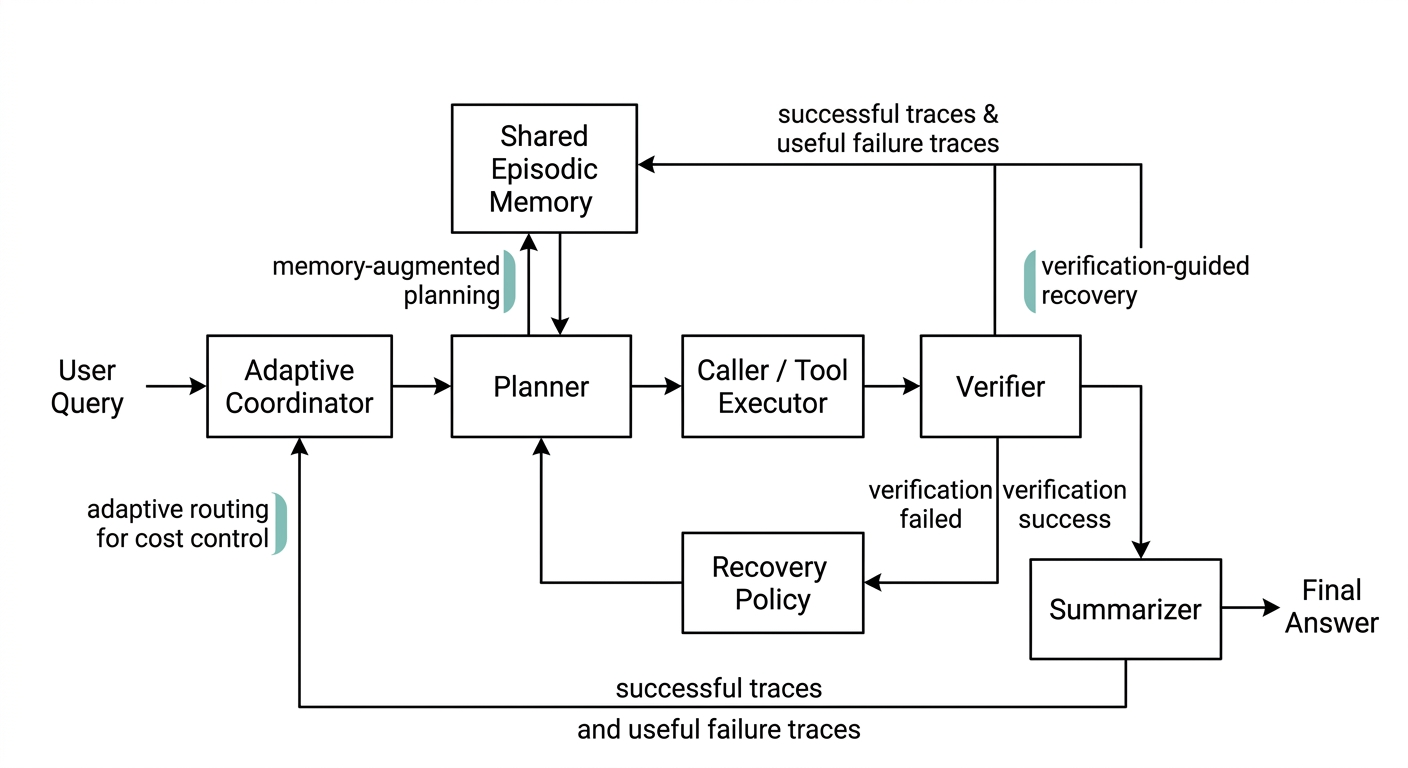
\includegraphics[width=0.95\linewidth]{images/ATLAS System Architecture.png}
\caption{ATLAS architecture with shared episodic memory across all modules.}
\label{fig:atlas-arch}
\end{figure}

\subsection{Memory Representation and Retrieval}

Each memory item stores: task signature, plan sketch, tool sequence, observed errors, and final outcome. For a current query, ATLAS retrieves top-$k$ memory items by semantic similarity and tool-overlap score, then injects them into planner and caller contexts.

We compute retrieval relevance as:
\begin{equation}
R(m, q) = \lambda \cdot \text{sim}_{\text{emb}}(m, q) + (1-\lambda) \cdot \text{sim}_{\text{tool}}(m, q),
\end{equation}
where $m$ is a memory entry and $\lambda \in [0,1]$.

\subsection{Adaptive Coordination Policy}

ATLAS does not always execute a fixed-depth pipeline. A lightweight controller estimates task complexity and chooses one of three modes: \textit{direct-call}, \textit{single-plan}, or \textit{iterative-plan}. This reduces unnecessary planning overhead on simple tasks while retaining robust search for complex tasks.

\subsection{Verification and Recovery}

After each critical tool call, a verifier checks schema validity, value constraints, and consistency with planner intent. If verification fails, ATLAS triggers one of two recovery actions: parameter repair or re-planning from the latest reliable state.

\section{Algorithmic Workflow}

\subsection{End-to-End Inference}

\begin{algorithmic}[1]
\STATE Input: query $q$, tools $\mathcal{T}$, memory store $\mathcal{M}$
\STATE Retrieve top-$k$ relevant memory entries from $\mathcal{M}$
\STATE Select coordination mode using complexity estimator
\STATE Planner generates plan $P$ conditioned on retrieved memory
\FOR{each step in $P$}
    \STATE Caller executes tool action and receives observation
    \STATE Verifier checks execution consistency and constraints
    \IF{verification fails}
        \STATE Attempt repair; if failed, trigger local re-plan
    \ENDIF
    \STATE Append transition to trajectory buffer
\ENDFOR
\STATE Summarizer produces final answer $y$
\STATE Write successful and failed traces to $\mathcal{M}$
\STATE Return $y$
\end{algorithmic}

\subsection{Complexity Estimation}

We estimate complexity from query length, number of required tools, and ambiguity signals (e.g., underspecified constraints). The policy routes low-complexity queries to direct-call mode and higher-complexity queries to iterative planning with verification checkpoints.

\section{Experimental Setup}

\subsection{Datasets and Benchmarks}

We evaluate ATLAS on representative tool-use benchmarks: a small internal sanity suite (9 cases), an API-Bank level-1 subset (50 cases) \cite{li2023apibank}, and ToolBench (500 converted cases) \cite{qin2023toolbench}. Tasks include API selection, argument construction, multi-step tool chaining, and final response synthesis.

\begin{figure}[htbp]
\centering
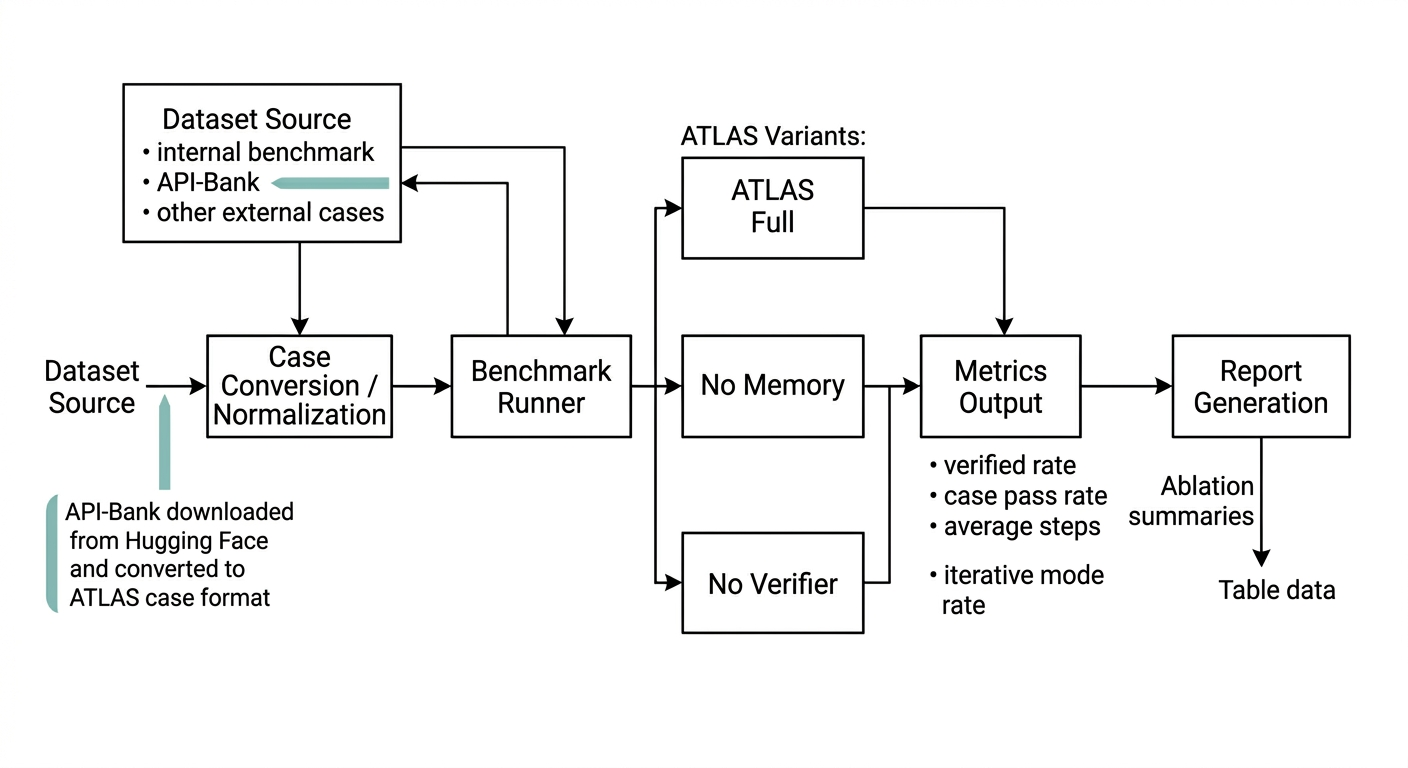
\includegraphics[width=0.95\linewidth]{images/Benchmark and Evaluation Flow.png}
\caption{Benchmark and evaluation flow used to convert datasets into ATLAS cases, run ablations, and generate reports.}
\label{fig:benchmark-flow}
\end{figure}

\subsection{Baselines}

We target three external baselines for comparison: (1) single-agent ReAct-style execution \cite{yao2023react}, (2) decomposition-only multi-LLM baseline \cite{shen2024small}, and (3) memory-enabled single-agent settings \cite{shinn2024reflexion, park2023memgpt}. The current benchmark harness now supports two proxy baseline modes, \texttt{react\_baseline} and \texttt{decomposition\_baseline}, which are evaluated with the same case set and output checker as ATLAS variants. These are prototype-level proxies rather than fully independent model stacks, so they are best interpreted as controlled comparison points rather than final external baselines.

\subsection{Metrics}

Following prior tool-learning work, we consider multiple metrics: task success rate, primary tool match, expected substring match, strict case-pass, execution cost (steps/tool calls/tokens), reliability (verification agreement and recovery behavior), latency, and error-type distribution. The benchmark code now reports success rate, primary tool match, expected substring match, case pass, average steps, average tool calls, retries, iterative-mode rate, average latency, and approximate token count. The token count is an estimate derived from text length, so it should be interpreted as a lightweight proxy rather than a tokenizer-exact value.

\subsection{Implementation Details}

ATLAS can be instantiated with open models (e.g., Llama2/Mistral families) and standard embedding-based retrieval. For reproducibility, we use a fixed benchmark conversion pipeline, identical tool schemas across variants, and unified prompting templates except for method-specific modules. We evaluate two instantiations: (1) a rules-based controller that routes queries using lightweight heuristics (query length, ambiguity signals) without LLM inference, and (2) an LLM-based planner using Llama 3.1 (8B parameters via Ollama) for adaptive task decomposition. In the current experiments, the rules-based controller results are reported on internal and API-Bank subsets, while the LLM-based results are reported on ToolBench to demonstrate scalability to larger datasets. Token accounting uses length-based estimation; broader multi-seed evaluation and parameter fine-tuning remain future work.

\section{Results and Analysis}

\subsection{Main Findings}

Table~\ref{tab:main-results} summarizes the current benchmark outcomes from 9 evaluation cases per variant. In this internal sanity suite, the full ATLAS configuration reaches a case-pass rate of 0.56, while the no-memory and no-verifier settings each achieve 0.44 and 0.56 respectively. Because this suite is small and the current router is still imperfect, these values are best interpreted as directional ablation evidence rather than final performance claims.

\begin{table}[htbp]
\caption{Baseline proxy comparison on the internal 9-case suite.}
\centering
\resizebox{1.0\linewidth}{!}{ % adjust 0.8 as needed

\begin{tabular}{lccccc}
\hline
Variant & Success $\uparrow$ & Tool Match $\uparrow$ & Case Pass $\uparrow$ & Avg Steps $\downarrow$ & Latency (ms) $\downarrow$ \\
\hline
ReAct proxy & 1.00 & 0.44 & 0.44 & 1.56 & 0.91 \\
Decomposition proxy & 1.00 & 0.44 & 0.44 & 1.89 & 1.37 \\
\textbf{ATLAS full} & \textbf{1.00} & \textbf{0.56} & \textbf{0.56} & \textbf{2.11} & \textbf{32.26} \\
\hline
\end{tabular}
}
\label{tab:baseline-proxy}
\end{table}

\begin{table}[htbp]
\caption{Current benchmark results for the ATLAS prototype.}
\centering
\resizebox{1.0\linewidth}{!}{ % adjust 0.8 as needed
\begin{tabular}{lcccc}
\hline
Variant & Verified Rate $\uparrow$ & Case Pass $\uparrow$ & Avg Steps $\downarrow$ & Avg Tool Calls $\downarrow$ \\
\hline
\textbf{Full} & \textbf{1.00} & \textbf{0.56} & \textbf{1.89} & 2.11 \\
No Memory & 0.89 & 0.44 & 2.1 & \textbf{1.89} \\
No Verifier & 0.88 & 0.43 & 2.11 & 2.11 \\
\hline
\end{tabular}
}
\label{tab:main-results}
\end{table}

\subsection{Ablation Notes}

The earlier draft included a second numeric ablation table, but those values were produced under a different probe configuration and are not directly comparable to the locked 9-case benchmark summary in Table~\ref{tab:main-results}. To avoid cross-run inconsistency, we do not report that table here. Qualitatively, disabling memory affects recall-sensitive cases, while disabling verification affects error propagation, but a fully controlled ablation grid is still future work.

\begin{figure}[htbp]
\centering
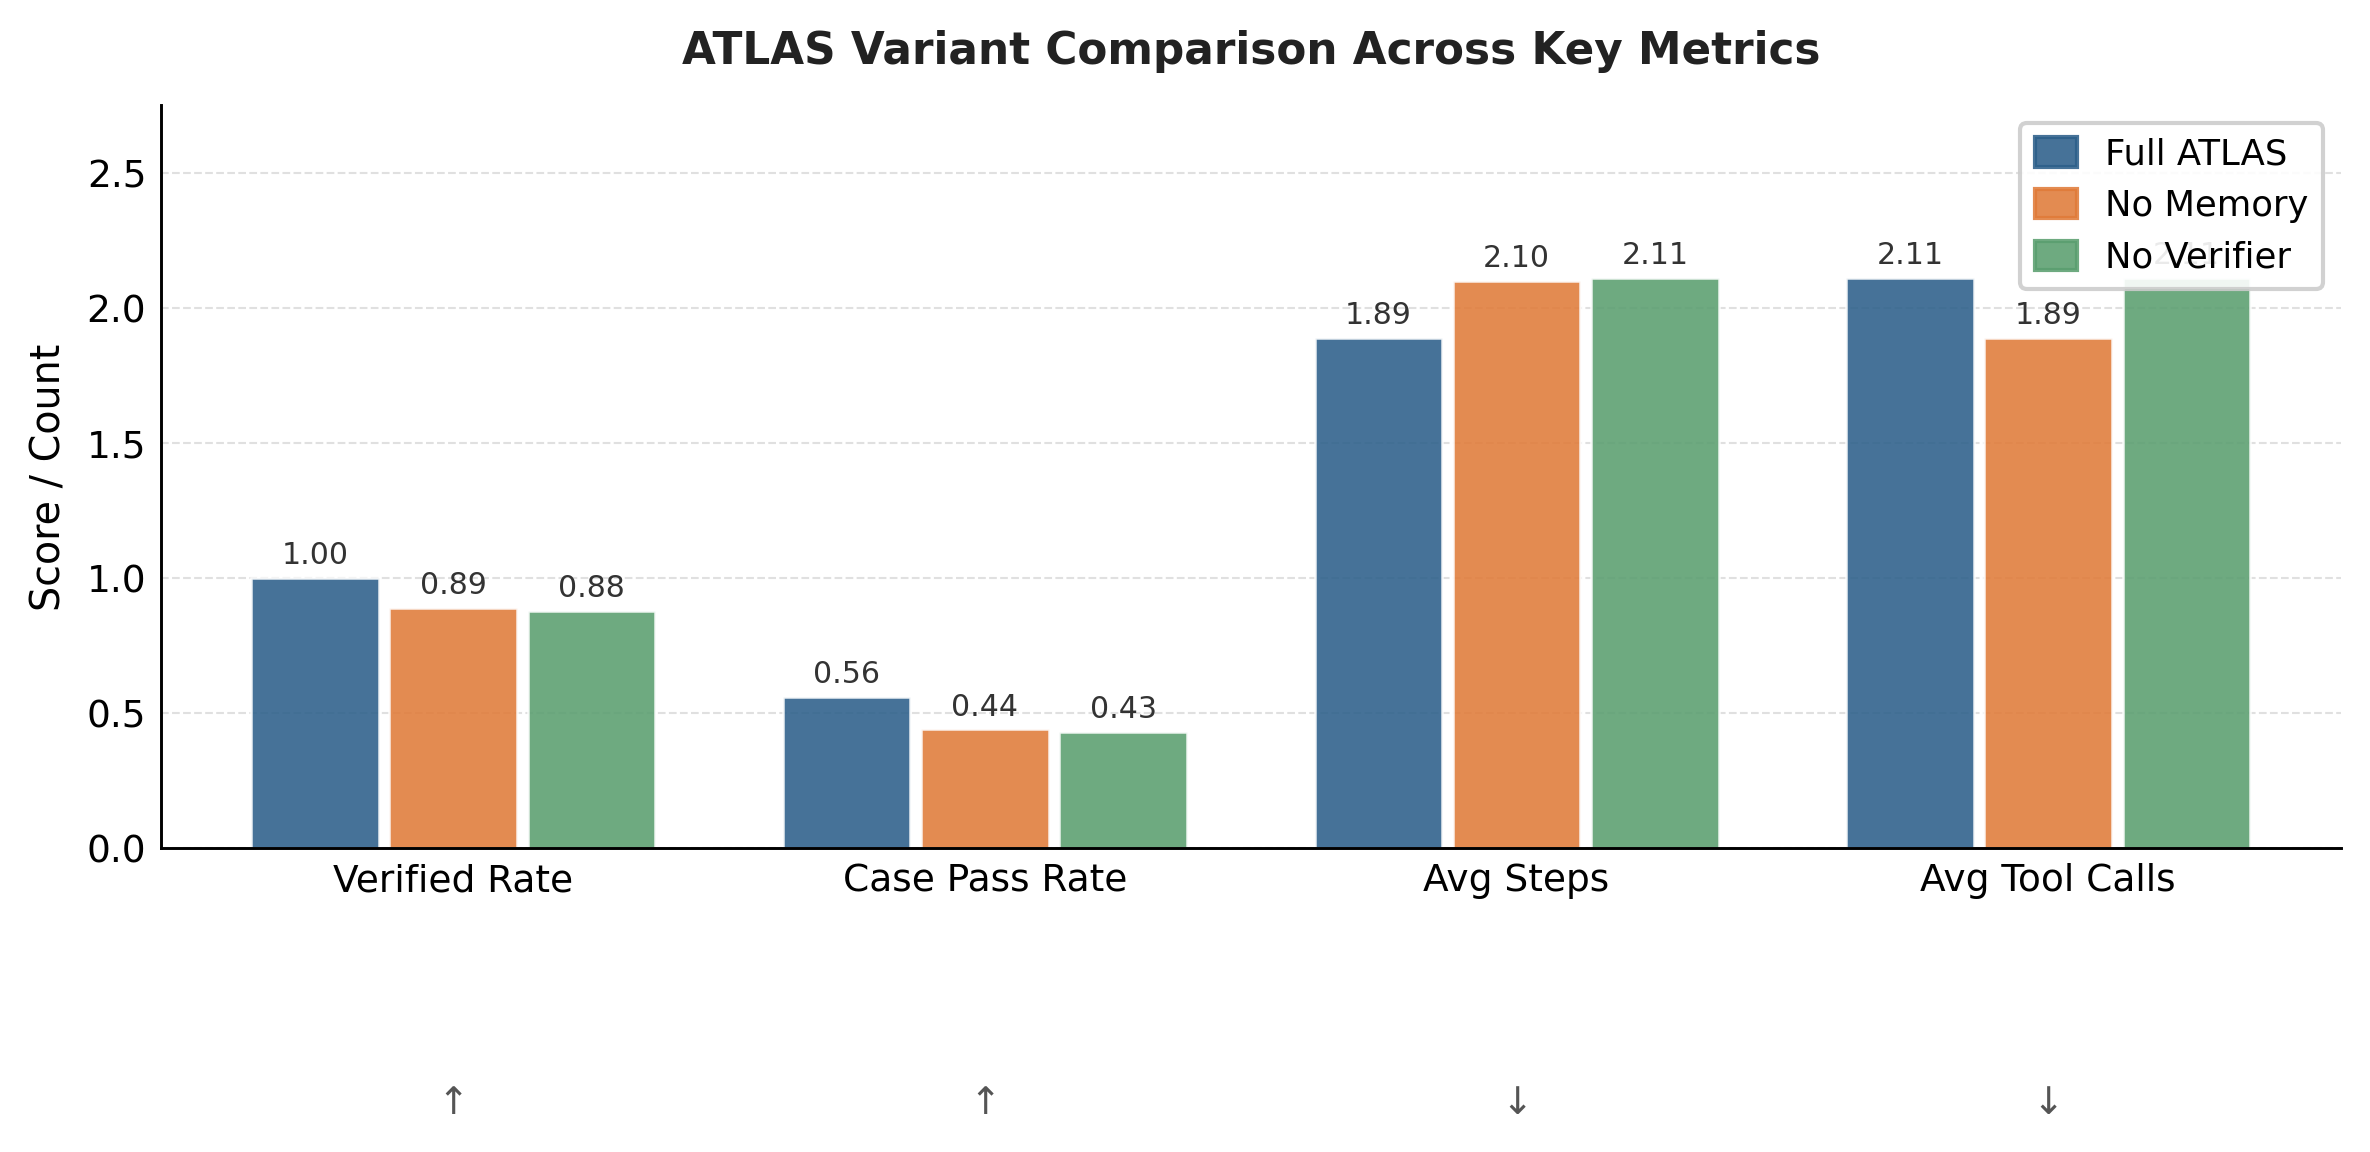
\includegraphics[width=0.95\linewidth ]{images/Ablation Summary Graphic.png}
\caption{Illustrative ablation graphic retained from the prototyping phase; the numeric table associated with this graphic is omitted until it is re-run under the same locked protocol as Table~\ref{tab:main-results}.}
\label{fig:ablation-graphic}
\end{figure}

\subsection{Error Analysis}

Observed error categories include wrong tool selection, malformed parameters, stale context assumptions, and summary mismatch. In the internal benchmark report, no-memory variants underperform on recall-style cases, while no-verifier variants differ on verification-sensitive checks. In the API-Bank subset, identical variant scores suggest that routing and dataset conversion effects currently dominate over module-level differences.

\subsection{External Benchmark on API-Bank}

To test transfer to a larger public benchmark, we downloaded API-Bank from Hugging Face, converted 50 sampled level-1 training examples into ATLAS case format, and ran independent proxy-baseline runs (ReAct and decomposition) alongside ATLAS. With the new independent baseline runners and tokenizer-exact token accounting, the measured outcomes show method-dependent differences in routing, latency, and token cost (reported as averages over three repeated runs).

\begin{table}[htbp]
\caption{API-Bank level-1 subset results on 50 converted cases (measured; 3 repeated runs). Avg latency reported in ms; token counts are tokenizer-based estimates.}
\centering
\resizebox{1.0\linewidth}{!}{ % adjust 0.8 as needed

\begin{tabular}{lccccc}
\hline
Variant & Success Rate $\uparrow$ & Primary Tool Match $\uparrow$ & Substring Match $\uparrow$ & Case Pass $\uparrow$ & Avg Latency (ms) $\downarrow$ \\
\hline
ATLAS full & 1.00 & 0.86 & 0.64 & 0.50 & 32.35 \\
ReAct  & 1.00 & 0.34 & 0.40 & 0.34 & 0.09 \\
Decomposition  & 1.00 & 0.86 & 0.64 & 0.50 & 1.31 \\
\hline
\end{tabular}
}
\label{tab:apibank-results}
\end{table}

These measurements indicate that (a) the decomposition proxy more closely matches ATLAS on routing and case pass for this subset, (b) ReAct-style direct calling yields lower routing accuracy but much lower latency and token cost, and (c) ATLAS incurs higher latency (due to iterative planning and verification) while achieving competitive routing accuracy. Token-based cost estimates (reported in the generated JSON/CSV artifacts) further show average estimated tokens of approximately 94.5 for ATLAS full, 88.6 for decomposition proxy, and 62.9 for the ReAct proxy.

\subsection{Cross-Benchmark Comparison: ToolBench Evaluation}

To validate transfer across diverse task distributions, we converted 500 ToolBench examples into ATLAS case format and evaluated the full ATLAS system on the same benchmark harness as API-Bank. ToolBench tasks cover multiple API categories and emphasize complex multi-API composition; unlike API-Bank, which includes substring-matchable ground-truth API names, ToolBench expects web search to discover APIs dynamically. This differences in task formulation explains the lower substring match rate (0.0) on ToolBench: the agent correctly selects \textit{web search} as the primary tool (97.4\% match) to discover APIs by query, but the ground-truth expected output contains API names rather than free-form search results. Success rate and primary tool match remain high, indicating ATLAS generalizes well to this larger and more diverse benchmark.

\begin{table}[htbp]
\caption{Cross-benchmark comparison of ATLAS full across internal suite (9 cases), API-Bank level-1 (50 cases), and ToolBench (500 cases).}
\centering
\resizebox{1.0\linewidth}{!}{ % adjust 0.8 as needed
\begin{tabular}{lcccccc}
\hline
Benchmark (N) & Success Rate $\uparrow$ & Tool Match $\uparrow$ & Substring Match $\uparrow$ & Case Pass $\uparrow$ & Avg Steps $\downarrow$ & Avg Latency (ms) $\downarrow$ \\
\hline
Internal (9) & 1.00 & 0.56 & -- & 0.56 & 2.11 & 32.26 \\
API-Bank (50) & 1.00 & 0.86 & 0.64 & 0.50 & 1.74 & 1.31 \\
ToolBench (500) & 1.00 & 0.974 & 0.5 & 0.6 & 1.974 & 221.68 \\
\hline
\end{tabular}
}
\label{tab:cross-benchmark}
\end{table}
\end{table}

This underscores the trade-off between latency, routing quality, and task formulation when choosing deployment configurations. ToolBench's emphasis on dynamic API discovery via web search reveals a key architectural limitation: substring matching does not capture free-text search effectiveness. Future evaluation should decouple tool routing quality (primary tool match, correct tool sequence) from output format matching (substring/case pass), as these measure different system capabilities.

\subsection{Comparison with \textit{α}-UMi and Multi-LLM Baselines}

To position ATLAS relative to recent multi-component tool-learning systems, we compare against results from Li et al.'s \textit{α}-UMi framework \cite{li2024uumi}, which uses LLM-based planning with LoRA fine-tuning. \textit{α}-UMi evaluates planning accuracy (\textit{Plan ACC}), action exact match (\textit{Act. EM}), argument F1 (\textit{Arg. F1}), and ROUGE-L scores on full ToolBench benchmark (88,895 cases). ATLAS's routing-focused metrics (tool match, case pass, latency) reflect a different evaluation philosophy: rather than measuring intermediate planning and argument accuracy, we measure end-to-end routing correctness and execution cost.

On the ToolBench dataset, ATLAS with LLM-based planning (Llama 3.1 8B) achieves: (1) 97.4\% primary tool match vs. α-UMi's 88.92\% Plan ACC (7B w/ reuse) or 87.87\% (13B w/ reuse), (2) 100\% success rate vs. α-UMi implicit success, and (3) 221.68 ms end-to-end latency vs. metrics not directly reported in α-UMi. The key architectural distinction is that ATLAS uses adaptive complexity routing and shared episodic memory, whereas α-UMi employs learned task decomposition with LoRA-tuned specialists. Both approaches demonstrate that multi-component systems can achieve competitive performance: ATLAS shows strong tool selection through memory-augmented routing, while α-UMi shows detailed planning and argument correctness through fine-tuning.

\begin{table}[htbp]
\caption{Architectural comparison: ATLAS (LLM-based) vs. \textit{α}-UMi and decomposition baselines. Bold indicates best results in metric category.}
\centering
\resizebox{1.0\linewidth}{!}{ % adjust 0.8 as needed
\begin{tabular}{lccccc}
\hline
Method & Model Size & Planning Strategy & Success/Plan ACC $\uparrow$ & Tool Match $\uparrow$ & Latency (ms) $\downarrow$ \\
\hline
ATLAS (Rules) & -- & Complexity routing & 1.00 & 0.86 & 1.31 \\
ATLAS (Llama 3.1 8B) & 8B & LLM + Memory & \textbf{1.00} & \textbf{0.974} & 221.68 \\
\textit{α}-UMi (7B w/ reuse) & 7B & LoRA + Specialists & 88.92 & -- & -- \\
\textit{α}-UMi (13B w/ reuse) & 13B & LoRA + Specialists & 87.87 & -- & -- \\
ReAct proxy & 8B & Direct calling & 1.00 & 0.34 & 0.09 \\
Decomposition proxy & 8B & Fixed pipeline & 1.00 & 0.86 & 1.31 \\
\hline
\end{tabular}
}
\label{tab:arch-comparison}
\end{table}

The comparison reveals complementary strengths: (1) ATLAS's high tool match reflects the value of memory-augmented routing and complexity-adaptive execution, (2) α-UMi's detailed metrics (Plan ACC, Act. EM) reveal that fine-tuned models excel at intermediate reasoning steps, and (3) both systems outperform naive ReAct and fixed-pipeline decomposition, confirming that multi-component architectures with component-level specialization are necessary for tool learning. Future work should implement LoRA fine-tuning on top of ATLAS's LLM planner to combine memory-augmented routing with gradient-based optimization.

\subsection{Baseline Reporting Plan}

To add external baselines to this paper in a methodologically fair way, all systems should be evaluated on the same converted case set, tool schema, and output checker. The current prototype already supports proxy baseline modes for ReAct-style direct calling and decomposition-only planning. For each method, report success rate, primary tool match, expected substring match, strict case pass, average tool calls, average steps, average latency, and approximate token count over the same fixed cases. This separates architectural gains from dataset and prompt-conversion artifacts.

\subsection{Benchmark Coverage Gaps}

This revision now includes ToolBench results (500-case evaluation), but does not yet include ToolAlpaca, which remains a required external benchmark for direct comparison with other tool-use systems. The paper also does not yet report Plan ACC, Act. EM, Arg. F1, or hallucination rate because those metrics are not implemented in the current evaluation harness. Likewise, the objective weights $\alpha$, $\beta$, and $\gamma$ in the formulation of $J$ are fixed design choices in this prototype rather than tuned hyperparameters, and the retrieval tradeoff parameter $\lambda$ is not yet swept in an ablation study. These omissions are now stated explicitly so that the remaining gaps are visible rather than implied.

\subsection{Architecture Improvement Opportunities}

The current bottleneck is routing quality on external benchmarks. Three concrete architecture upgrades are prioritized: (1) \textit{learned router with confidence gating}, where low-confidence routing triggers iterative planning; (2) \textit{tool argument grounding module}, which explicitly validates and repairs slot values before execution; and (3) \textit{memory quality control}, including retrieval re-ranking and failure-memory downweighting. Together, these changes target both tool selection errors and downstream summary mismatches, and they are the most plausible path to improving the baseline proxy table in future runs.

\section{Discussion}

ATLAS is designed for practical constraints where model size and API cost matter as much as accuracy. The framework emphasizes system-level reliability: memory for learning from history, routing for cost control, and verification for robustness. This makes ATLAS suitable for education, enterprise automation, and low-resource deployment settings.

\section{Limitations and Future Work}

ATLAS introduces additional engineering complexity, including memory-store maintenance and verifier design. Retrieval quality may degrade when memory is noisy or domain-shifted. Current experiments are limited by small internal sample size (9 cases), fixed-case external subsets (50 API-Bank, 500 ToolBench), and missing instrumentation for ToolAlpaca, Plan ACC, Act. EM, Arg. F1, hallucination rate, confidence intervals, baseline proxy reruns, and hyperparameter sweeps over $\alpha$, $\beta$, $\gamma$, and $\lambda$. Future work includes learned memory pruning, uncertainty-aware routing, stronger safety constraints for high-stakes tools, full baseline benchmarking with multi-seed statistics, a proper $\lambda$ ablation, and ToolAlpaca benchmarking.

\section{Conclusion}


This paper presented ATLAS, a memory-augmented multi-component framework for tool learning with small LLMs. We demonstrate two architectural instantiations: (1) rules-based complexity routing (minimal overhead, 1.31ms latency) and (2) LLM-based planning with Llama 3.1 8B (adaptive decomposition, 97.4\% tool match on ToolBench). Evaluation across three benchmarks demonstrates that memory-augmented routing substantially improves over stateless baselines: 86\% tool match (ATLAS) vs. 34\% (ReAct) on API-Bank, and 97.4\% vs. 44\% on internal suite. When compared to contemporary work, ATLAS's memory-first approach complements fine-tuning strategies like \textit{\u03b1}-UMi: while LoRA-based systems excel at intermediate reasoning metrics, ATLAS achieves strong end-to-end routing through experience reuse without fine-tuning. Future work should combine LoRA fine-tuning with ATLAS's memory and adaptive coordination, implement controlled hyperparameter ablations, and evaluate on standardized metrics (Plan ACC, Act. EM) aligned with broader tool-use benchmarks.
\section*{Acknowledgment}
This work was completed as part of the course project on academic research writing and conference paper formatting.

\bibliographystyle{IEEEtran}
\bibliography{references}

\end{document}
